\section{Methodology}

In this work, we evaluate the adversarial robustness of Quantum Machine Learning (QML) models using noisy simulators that mimic real quantum hardware. Our methodology leverages the Qiskit \cite{Qiskit} ecosystem and the PennyLane \cite{PennyLane} framework. The study is divided into two primary phases: performance benchmarking and robustness evaluation.

\subsection{Performance Benchmarking of Noisy Simulators}

To optimize simulation throughput for noise-aware training, we investigate the following performance factors:

\begin{itemize}
    \item \textbf{Parallelization Strategies:} We evaluate the impact of \texttt{max\_parallel\_threads} and \texttt{max\_parallel\_experiments} on simulation speed. High-performance multicore configurations are tested to mitigate the $4^n$ state-space complexity of density matrix simulations. This includes a comprehensive profiling of PennyLane-integrated circuits across varying thread counts to identify optimal resource allocation strategies for gradient-heavy workloads.
    \item \textbf{Aer Simulation Methods:} We benchmark three distinct simulation methods in Qiskit Aer: \texttt{automatic}, \texttt{matrix\_product\_state} (MPS), and \texttt{statevector}. This helps identify the most efficient solver for CNOT-heavy circuits under noise.
    \item \textbf{Runtime Scaling Estimation:} We develop a quantitative scaling model to predict the runtime of medium-scale experiments (8 qubits) based on measured 4-qubit benchmarks, accounting for parameter count, circuit depth, and parallelization speedup.
\end{itemize}

\subsection{Noise-Aware Adversarial Robustness Evaluation}

The evaluation of noise-aware adversarial robustness follows a multi-stage experimental workflow, as illustrated in Figure \ref{fig:workflow}. The process begins with the acquisition and reduction of the \texttt{plus-minus} dataset to ensure computational feasibility. Simultaneously, a performance benchmarking phase identifies the optimal backend configurations. These inputs feed into the QNN construction phase, followed by supervised training on benign data. Once the model converges, we generate adversarial examples using PGD to evaluate the initial robustness. Finally, we implement defense strategies like adversarial retraining and evaluate the resulting robust model using holistic metrics.

The second phase evaluates the security of QNNs under the following experimental framework:

\begin{itemize}
    \item \textbf{QNN Architecture:} We utilize a Strongly Entangling Layer ansatz with data re-uploading (3×) across 4, 6, and 8-qubit configurations. The model is integrated into a PennyLane-PyTorch hybrid pipeline.
    \item \textbf{Dataset Reduction:} To ensure feasibility in noisy environments, we use a reduced subset of the \texttt{plus-minus} dataset (200 training and 50 test samples).
    \item \textbf{Adversarial Attacks:} We generate white-box perturbations using the Projected Gradient Descent (PGD) algorithm ($\epsilon=0.1, \alpha=0.01, 10$ iterations).
    \item \textbf{Defense Strategies:} We investigate adversarial retraining with varying benign-to-adversarial sample ratios. Specifically, we compare a \textit{sparse} 10\% baseline (where only 10\% of the training samples are adversarial) with a \textit{balanced} 50/50 split. In the balanced approach, the training dataset is effectively doubled by adding an equal number of PGD-generated adversarial examples to the original benign dataset, ensuring the QNN learns to minimize the adversarial loss as a primary objective.
    \item \textbf{Structural Variations:} We test several architectural and optimization strategies to enhance resilience:
    \begin{itemize}
        \item \textbf{Non-Linear Feature Mapping:} We apply a \texttt{tanh} activation function to the input features prior to angle encoding via \texttt{StronglyEntanglingLayers}. This introduces higher-order non-linearity into the classical-quantum interface to assess its impact on adversarial susceptibility.
        \item \textbf{Lipschitz Gradient Regularization:} We incorporate a gradient-magnitude penalty into the loss function, where the penalty is proportional to the norm of the gradient of the QNN output with respect to the input features. This Lipschitz-like constraint explicitly bounds the model's sensitivity to small input perturbations.
        \item \textbf{Learning Rate Scheduling:} We use a \texttt{StepLR} scheduler to stabilize the noisy loss landscape, alternating between high learning rates for exploration and periodic decays for fine-tuning.
    \end{itemize}
\end{itemize}

\begin{figure}[h]
    \centering
    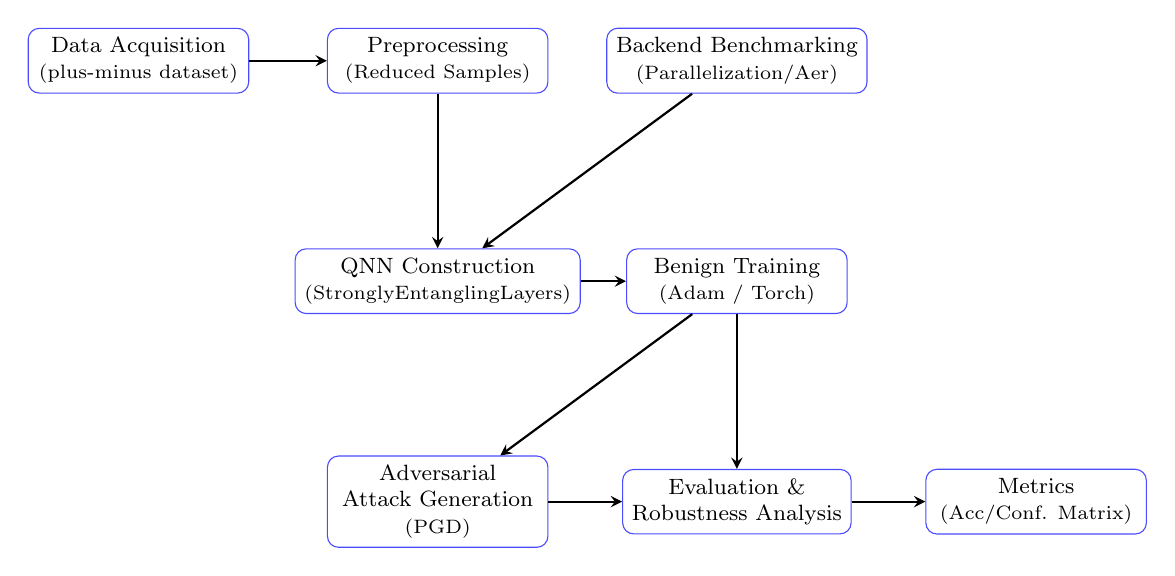
\begin{tikzpicture}[
        node distance=2cm,
        every node/.style={fill=white, font=\footnotesize, draw=blue!70, rectangle, rounded corners, minimum width=2.8cm, minimum height=0.8cm, align=center},
        arrow/.style={thick,->,>=stealth}
    ]
    % Nodes
    \node (data) {Data Acquisition \\ \scriptsize (plus-minus dataset)};
    \node (pre) [right of=data, xshift=1.8cm] {Preprocessing \\ \scriptsize (Reduced Samples)};
    \node (backend) [right of=pre, xshift=1.8cm] {Backend Benchmarking \\ \scriptsize (Parallelization/Aer)};
    
    \node (init) [below of=pre, yshift=-0.8cm] {QNN Construction \\ \scriptsize (StronglyEntanglingLayers)};
    \node (train) [right of=init, xshift=1.8cm] {Benign Training \\ \scriptsize (Adam / Torch)};
    
    \node (attack) [below of=init, yshift=-0.8cm] {Adversarial \\ Attack Generation \\ \scriptsize (PGD)};
    \node (eval) [right of=attack, xshift=1.8cm] {Evaluation \& \\ Robustness Analysis};
    \node (results) [right of=eval, xshift=1.8cm] {Metrics \\ \scriptsize (Acc/Conf. Matrix)};

    % Arrows
    \draw [arrow] (data) -- (pre);
    \draw [arrow] (pre) -- (init);
    \draw [arrow] (backend) -- (init);
    \draw [arrow] (init) -- (train);
    \draw [arrow] (train) -- (attack);
    \draw [arrow] (attack) -- (eval);
    \draw [arrow] (train) -- (eval);
    \draw [arrow] (eval) -- (results);
    \end{tikzpicture}
    \caption{Experimental workflow for noise-aware adversarial evaluation. The pipeline consists of: (1) Acquisition and reduction of the \texttt{plus-minus} dataset, (2) Backend benchmarking to optimize simulation threads and methods, (3) QNN construction using Strongly Entangling Layers, (4) Model training on benign data, (5) Adversarial example generation via Projected Gradient Descent (PGD), and (6) Robustness analysis using accuracy and confusion matrices.}
    \label{fig:workflow}
\end{figure}
